\documentclass{article}
\usepackage[left=35mm,margin=20mm]{geometry}
\usepackage{ifthen,empheq}
\usepackage{dot2texi}
\date{\today}
\usepackage{fancyhdr}
\usepackage{tikz}
\usepackage{listings}
\usetikzlibrary{calc,graphs,arrows}
\setlength{\headheight}{15pt}

\lhead{Assignment 1}
\chead{Dilawar Singh}
\rhead{\today}

\lfoot{}\cfoot{\thepage}\rfoot{}
\pagestyle{fancy}

\ifx\pdfoutput\undefined                         %LaTeX
  \RequirePackage[ps2pdf,bookmarks=true]{hyperref}
  \hypersetup{ %
    pdfauthor   = {\@author},
    pdftitle    = {\@title},
    pdfcreator  = {LaTeX with hyperref package},
    pdfproducer = {dvips + ps2pdf}
  }
\else                                            %PDFLaTeX
  \RequirePackage[pdftex,bookmarks=true]{hyperref}
  \hypersetup{ %
    pdfauthor   = {\@author},
    pdftitle    = {\@title},
    pdfcreator  = {LaTeX with hyperref package},
    pdfproducer = {dvips + ps2pdf}
  }
\pdfadjustspacing=1
\fi

% Set up counters for problems and subsections

\newcounter{ProblemNum}
\newcounter{SubProblemNum}[ProblemNum]

\renewcommand{\theProblemNum}{\arabic{ProblemNum}}
\renewcommand{\theSubProblemNum}{\alph{SubProblemNum}}

\newcommand*{\anyproblem}[1]{\newpage\subsection*{#1}}
\newcommand*{\problem}[1]{\stepcounter{ProblemNum} %
   \anyproblem{Problem \theProblemNum. \; #1}}
\newcommand*{\soln}[1]{\subsubsection*{#1}}
\newcommand*{\solution}{\soln{Solution}}
\renewcommand*{\part}{\stepcounter{SubProblemNum} %
  \soln{Part (\theSubProblemNum)}}

\renewcommand{\theenumi}{(\alph{enumi})}
\renewcommand{\labelenumi}{\theenumi}
\renewcommand{\theenumii}{\roman{enumii}}
\begin{document}

\problem{Decoding}

Consider the following set of codewords:

(A,B,C,D,E,F,G,H) = (01, 11, 001, 0000, 0001, 1001, 1010, 1011).

\begin{enumerate}
    \item Is this an instantaneous (prefix) code?
    \item Verify that it satisfies the Kraft inequality.
    \item Construct a string which has no meaning under this system Transmitting
        information across a channel.
\end{enumerate}

\solution

\part 

Yes. Function {\tt solvea} figures out if any code is a prefix of any other
code. The answer is that there is no code which prefix of any other code. Some
relevant snippet from the code is following.

\begin{verbatim}
*Main> alphabets 
"ABCDEFGH"
*Main> allcodes 
["01","11","001","0000","0001","1001","1010","1011"]
*Main> map isPrefixCode alphabets 
[False,False,False,False,False,False,False,False]
\end{verbatim}

\part

Function {\tt kraft } verifies that it is true. Following is the execution.

\begin{verbatim}
*Main> kraft_sum 
0.9375
*Main> kraft
True
*Main> 
\end{verbatim}

\part

Any string which function {\tt decoder} can't decode would have no meaning. Here
are some examples:

\begin{verbatim}
*Main> decode "101000101" 
"GCA"
*Main> decode "101000101111" 
"GCAB*** Exception: No valid alphabet for "1"
*Main> decode "1010001011110" 
"GCAB*** Exception: No valid alphabet for "10"
*Main> 
\end{verbatim}

\problem{} Consider the discrete memoryless channel Y = X + Z (mod 11), where Z
is uniformly distributed on the alphabet {1, 2, 3}, and $X \in \{0, 1, \ldots
10\}$ . Assume that Z is independent of X.

\begin{enumerate}
    \item Find the capacity.
    \item What is the maximizing $p^\star(x)$?
\end{enumerate}

\solution

\begin{figure}[ht!]
\begin{center}
    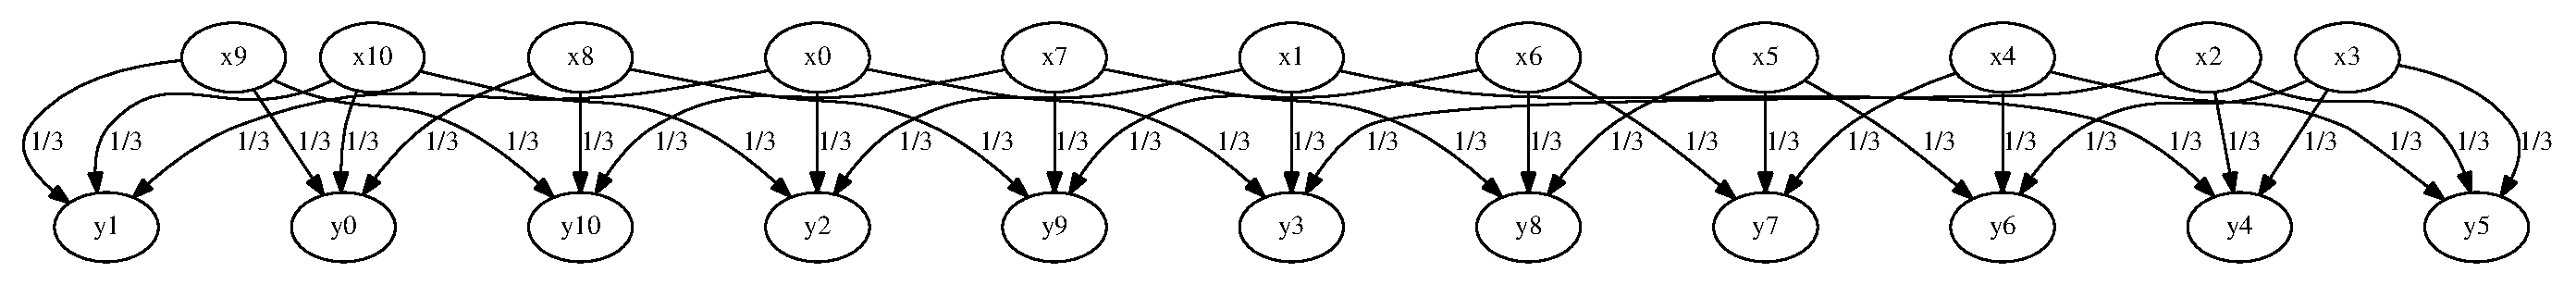
\includegraphics[width=1.0\textwidth]{_images/channel.eps}
\end{center}
\caption{Channel with their input and output symbols.}
\end{figure}


\part During coding, all $x \in X$ goes to $x+1, x+2, x+3$ (mod 11) respectively
with probability 1/3. We consider two possibilities, we can send either \{0, 3,
6, 9\} with the possibility of  $9 \rightarrow 1$ and $0 \rightarrow 1$. Or we
can drop 0 or 9 from the set. In the former, we can send one of 4 symbols per
transmission with a small probability of error (i.e. $9 \rightarrow 1$ and $0
\rightarrow 1$); in later case, we can send one of the 3 symbols per
transmission without any error but we will never send some symbols. None of
these situations are desirable. These argument  put some limit on channel
capacity, between $log_2 4 = 2$ and $log_2 3 = 1.5849$. 

This channel can be simplified to the following.
\begin{figure}[ht!]
\begin{center}
    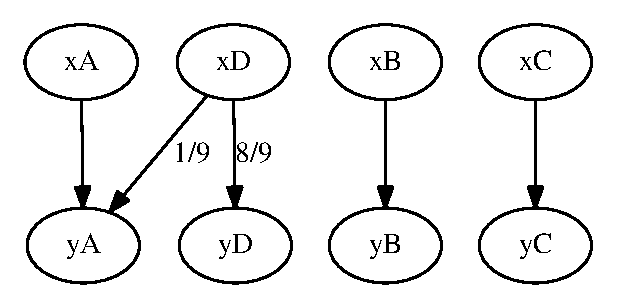
\includegraphics[width=0.4\textwidth]{_images/channel_simple.eps}
\end{center}
\caption{}
\end{figure}

Since we know the binary symmetric channel, we can further approximate the
binary asymmetric channel with a symmetric one to get another approximation of
mutual information under given distribution of $X$.

$ I(X; Y) = log_2 {2} + (1 - H(\frac{1}{9})) = 1 + 0.6477 = 1.6477 $

The python listing in appendix, shows how mutual information converges to a
value (approx 1.84) during simulation as we increases the size of input
sequences. This matches well with the derivation of maximum capacity of a binary
asymmetric channel on Wikipedia i.e. $1 - 0.5 H(\frac{1}{9})$ when input follows
a Bernoulli distribution.

We can also derive the expression for maximum capacity.

\begin{align}
I(Y;X) &= H(Y) - H(Y|X) = H(Y) - H(X+Z|X) = H(Y) - H(Z|X) = H(Y) - H(X) \\
    &= H(Y) - log_2 3 \\
\max I(Y; X) &= \max H(Y) - log_2 3
\end{align}

Which is achieved when Y is uniformly distributed. The channel capacity in this
case is $log 11 - log 3 = 1.8744$.



\begin{verbatim}
Computing for sequence of length 49238.8263171 
[INFO] Initializing channel
[INFO] Total 11 input symbols, total 11 output symbol
|- Mutual info 1.8428914487
Computing for sequence of length 62355.0734127 
[INFO] Initializing channel
[INFO] Total 11 input symbols, total 11 output symbol
|- Mutual info 1.84410956054
Computing for sequence of length 78965.228685 
[INFO] Initializing channel
[INFO] Total 11 input symbols, total 11 output symbol
|- Mutual info 1.84348815998
Computing for sequence of length 100000.0 
[INFO] Initializing channel
[INFO] Total 11 input symbols, total 11 output symbol
|- Mutual info 1.84570556055
\end{verbatim}

\begin{figure}[ht!]
\begin{center}
    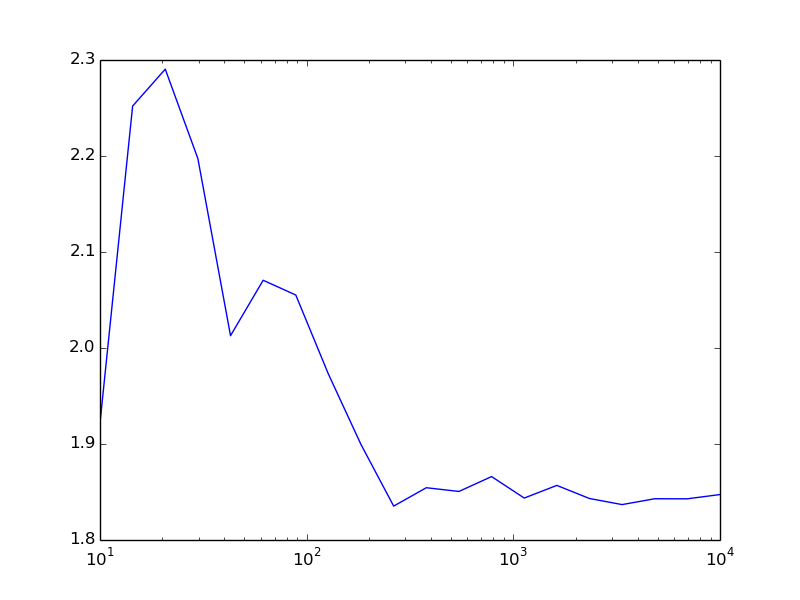
\includegraphics[width=\textwidth]{./mutual_info.png}
\end{center}
\caption{Mutual information of channel with size of input sequences}
\end{figure}


\problem{}

The Z channel has binary input and output alphabets and transition
probabilities $p(y|x)$ given by the following matrix: Q =

\begin{tabular}{c c c}
 & 1 &  0 \\
 &1/2 & 1/2 \\
\end{tabular}

$x, y \in \{0, 1\}$.

[Why is it called the Z-channel?] . Because it looks like Z 

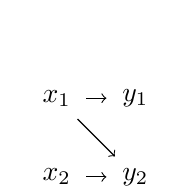
\begin{tikzpicture}[scale=1, every node/.style={circle} ]

    \node[] (a) at (0,0) {$x_1$};
    \node[right of=a]  (b) {$y_1$};
    \node[below of=a]  (c) {$x_2$};
    \node[below of=b]  (d) {$y_2$};
    \draw[->] (a) -- (b);
    \draw[->] (a) -- (d);
    \draw[->] (c) -- (d);

\end{tikzpicture}    

Find the capacity of the Z channel and the maximizing input probability
distribution.

\solution

The joint probability distribution of channel is below when $p(X=X_1) = \alpha$.

\begin{tabular}{c | c c}
    & $Y_1$ & $Y_2$ \\
    \hline 
    $X_1$ & $\alpha$ & 0 \\
    $X_2$ & $(1-\alpha)/2$ & $(1-\alpha)/2$ \\
    \hline
\end{tabular}

And, 

\begin{align}
I(Y;X) &= H(Y) - H(Y|X) \\
    &= H\left(\frac{1-\alpha}{2}\right) - (1 - \alpha) \\
\end{align}

To find a maximum, we use elementary calculus with the variable substitution
$\beta = 1 - \alpha$.

\begin{align}
    I(\beta) &= H(\beta/2) - \beta  \\
    &= 1 - \frac{\beta \log(\beta)}{2} - \log(2 - \beta) +
    \frac{\beta\log(2-\beta)}{2} - \beta \\
\end{align}

$I(\beta=0)$ and $I(\beta=1)$ is 0 while the function $I$ takes positive values
for some $\beta \in (0, 1)$. Therefore it must have at least one maxima in
interval $\beta \in (0, 1)$. To find it, we set the first derivative i.e.
$\frac{dI}{d\beta} = 0$.

\begin{align}
    \frac{dI}{d\beta} &= 0 \\
    \frac{-1}{2}\left( 1 + \log \beta \right) + \frac{1}{2-\beta} + \frac{1}{2}
    \left( \frac{-\beta}{2-\beta} + \log (2 - \beta) \right) -1 &= 0 \\
    \frac{1}{2} \log \frac{2-\beta}{\beta} &= 1 \\
    \beta &= \frac{2}{5}
\end{align}

The value of $I(Y;X)$ at $\beta=\frac{2}{5}$ is $\log 5 - 2 = 0.3219$. Let's see
what the simulator says:


\problem{}

[Optional] For the Z channel of the previous problem, assume that we choose a
($2^{nR}$) code at random, where each codeword is a sequence of fair coin
tosses. This will not achieve capacity. Find the maximum rate R such that the
probability of error $P_e^n$ , averaged over randomly generated codes, tends to
zero as the block length n tends to infinity.

\appendix
\section{Haskell listing}

\section{Python listing}
%\begin{lstlisting}
\lstinputlisting[firstline=15,language=python]{channel.py}
%\end{lstlisting}
\end{document}
